%%%%%%%%%%%%%%
% Fichero: principal.tex
% Autor: Jesús Salido Tercero (https://www.esi.uclm.es/www/jsalido)
% Fecha (creación): febrero 2010 
% Rev. : abril 2025
% Descripción: Plantilla para memoria de TFG 
% (Escuela Sup. de Informática, UCLM). Creada para el curso 
% “LaTeX esencial para preparación de TFG, Tesis y otros documentos 
% académicos” (Esc. Sup. Informática-UCLM)
%
%### Compilación 
%
% Esta plantilla ha sido preparada para compilarse con `pdflatex`  
% (bibliografía con `bibtex`). Se recomienda emplear una distribución
% de LaTeX como MiKTeX o TeXLive.
%
% Una versión revisada de esta plantilla está disponible en Overleaf para
% trabajar online. 
%
% Si deseas acceder a la versión de desarrollo puedes encontrarla en GitHub:
%	https://github.com/JesusSalido/TFG_ESI_UCLM
%%%%%%%%%%%%%%

% Al llamar a la clase puedes pasarle opciones que indican el idioma pral.
% del documento (spanish o english), el tipo de dispositivo (normal, para 
% imprimir en papel y screen para leer en pantalla), y si se desea
% numeración de páginas en el pie (pageonfooter=true) o en la cabecera
% (pageonfooter=false).
\documentclass[final, % final o draft (sin figuras)
				english, % Idioma pral. (spanish o english)
				device=screen, % Tipo de dispositivo (normal o screen)
				pageonfooter=false % Paginación en el pie
]{TFGesi}

% -------------------------
% EDITA: Los datos del documento con la información de tu trabajo.
%
% IMPORTANTE: Todos los campos son obligatorios, 
% pero \cotutline se puede dejar vacío.
%
% Algunos datos deben declararse en el idioma alternativo al pral.
% del documento. Estos datos se emplean en el resumen en el idioma
% alternativo.  
%
% La clase TFGesi los usa para generar el contenido personalizado.
% Puedes usarlos en cualquier parte del documento suprimiendo 
% el carácter '@', p.ej., \titulo
% -------------------------
\makeatletter 
\@titulo{MADTrack: Distributed System for Dataset and Artificial Intelligence Model Management} % 1ª Línea
\@tituloCorto{MADTrack: SD de gestión de conjuntos de datos y modelos de IA} % En idioma pral.
\@tituloCortoAlt{MADTrack: DS for Dataset and AI Model Management} % En idioma alt.
\@autoria{Miguel Ángel Ruiz Arreaza}
\@email{miguelangel.ruiz9@alu.uclm.es}
\@autorline{Author: \autoria}
\@tutline{Tutor: José Luis Espinosa Aranda}
\@cotutline{Co-tutor: Pablo Tomás Toledano González}
%\@cotutline{} % Si no procede dejar vacío (NO BORRAR)
\@instEdu{UNIVERSIDAD DE CASTILLA-LA MANCHA}
\@centroEdu{ESCUELA SUPERIOR DE INFORMÁTICA}
\@titulacion{BACHELOR IN COMPUTING ENGINEERING} % En idioma pral.
\@titulacionAlt{GRADO EN INGENIERÍA INFORMÁTICA} % En idioma alt.
\@especialidad{Coursed intensification: Computer Engineering} 
\@depto{Tutor's Department: }
\@tipoDoc{BACHELOR DISSERTATION} % En idioma pral.
\@tipoDocAlt{TRABAJO FIN DE GRADO} % En idioma alt.
\@mesTF{Julio}        	% Mes de defensa
\@monthTF{July}        	% En inglés
\@yearTF{2025}        	% Año de defensa
\@cityTF{Ciudad Real}	% Ciudad de defensa
\@escudo{esiLogo}       % Logo centro (pdf, png o jpg)
\makeatother 
% -------------------------

% Palabras clave: Son importantes para facilitar búsqueda en Internet
% Se añaden como metadatos al PDF final.
\setkeywords{% (hasta 5 o 6 máx.)
	Escuela Superior de Informática, %
	UCLM, %
	TFG, %
	\LaTeX, %
	\TeX Live, %
	AI, %
	Deep Learning, %
	Distributed System, %
	Dataset, %
	configuration management %
} 

% -------------------------
% CARGAR GLOSARIO
% -------------------------
\makeglossaries

% -------------------------
% CUERPO del documento
% -------------------------
% Para pruebas, limita los ficheros incluidos.
%\includeonly{} 
\begin{document}

\newacronym{AI}{AI}{Artificial Intelligence}
\newacronym{CV}{CV}{Computer Vision}

% -------------------------
% ACRÓNIMOS
% -------------------------
%%\newacronym{DS}{DS}{Distributed Systems}
%%\newacronym{AI}{AI}{Artificial Intelligence}
%%\newacronym{DL}{DL}{Deep Learning}
%%\newacronym{NN}{NN}{Neural Network}


% -------------------------
% Portadas, créditos, resumen, agradecimiento, notación e índices. 
\frontmatter
%\input{./Anexos/PortadaETSII} % Por ej.,: Otras portadas
%\includepdf{fichero_portada.pdf} % Incluso como fichero PDF

% -------------------------------------------------------------------------
% PORTADA PRAL. (1)
% -------------------------------------------------------------------------

% \portadaOld % Portada pral.
\portadaNew

% -------------------------------------------------------------------------
% PORTADA INTERIOR (2)
% -------------------------------------------------------------------------
\portadaInt %Portada interior


% -------------------------
% CRÉDITOS
% -------------------------
\begin{creditos}[\titulo] % Editar a conveniencia (se pasa el título deseado)
The author may choose the license type they wish. This document is distributed under license CC BY-NC-SA 4.0. The full text of the license is available at \url{https://creativecommons.org/licenses/by-nc-sa/4.0/}. The copy and distribution of this work is permitted in all parts of the world, without royalties and in any medium, as long as this notice is preserved. In addition, permission is granted to copy and distribute translations of this book from the English original to another language, provided that the copyright notice and this permission notice are preserved in all copies.

\noindent \includegraphics[width=0.15\linewidth]{by-nc-sa}

% Para citar este plantilla empleando bibtex puedes emplear el registro siguiente:
%@www{salidoTFG,
%  author       = {Jesús Salido},
%  title        = {Plantilla guía de TFG para la ESI-UCLM},
%  year         = {2019},
%  editor       = {GitHub},
%  organization = {Universidad de Castilla-La Mancha},
%  url          = {https://github.com/JesusSalido/TFG_ESI_UCLM},
%  doi          = {10.5281/zenodo.4574562}
%}
\end{creditos}


% -------------------------
% CALIFICACIÓN DEL TRIBUNAL  (No necesario en versión electrónica)
% -------------------------
%\tribunal % Página opcional para calificación 


% -------------------------
% DEDICATORIA 
% -------------------------
\begin{dedicatoria} % (no confundir con los agradecimientos)
\emph{To my family, close friends, fellow colleagues, classmates and professors \\ % A alguien muy especial
For their patience and for accompanying me and showing me the way through this exciting journey.}
\end{dedicatoria}

\pagestyle{plain}	% Páginas sólo con numeración inferior al pie


% -------------------------
% RESÚMENES:
% -------------------------

% EDITAR: Resumen en idioma alternativo default=english (máx. 1 pág.)
%---
\begin{resumenAlt}[english]{\tituloCortoAlt} 
% Se pasa el idioma (opcional) y título

\emph{<<What>>}

Artificial Intelligence is on the rise, and many companies are striving to create a wide-ranging variety of models to help themselves and their customers in an equally wide range of specific tasks. This inevitably translates into multiple model trainings being performed a year and, in many cases, many datasets being created or modified in the same time interval. 
Such is the case of UBOTICA Technologies: a Space:AI company that works in Computation \emph{on the edge}, delivering AI solutions integrated in embedded systems incorporated in spatial modules, which come with limited space for storing data and computing power. The development of these solutions requires multiple training and deployment iterations,
which over the years presented challenges in maintaining optimal traceability across their AI training environments, increasing the time required to search for a specific AI training configuration. 


\emph{<<How>>}

MADTrack is a distributed configuration management system with the purpose of putting order to the aforementioned challenges. It will store, track and manage all changes within datasets and AI model configurations. The main 
restrictions over the development of the system are the limited storage space of the company for this resources (the management of the evolution of datasets and models has to be done efficiently), the distributed nature of the environment where the items 
are stored and managed and the need for the system to be integrated in a greater processing workflow. The development of the system will be divided in a series of prototypes with an iterative and incremental approach, following continuous testing policies.



\emph{<<Conclusion>>}

The resulting system will consist of a distributed system following the client-server application, with a local or remote server attending requests from multiple clients sending requests by means of a software wrapper library which in turn will interact with other open-source technologies.

\end{resumenAlt}

% EDITAR: Resumen en idioma pral. default=spanish (máx. 1 pág.) 
\begin{resumenPral}[spanish]{\titulo} % Se pasa el idioma (opcional) y título

\emph{<<Que>>}

La Inteligencia Artificial está en ascenso, y muchas empresas están trabajando en la elaboración de una inmensa variedad de modelos que las ayuden tanto a ellas 
como a sus clientes a realizar una variedad de tareas igualmente amplia. Esto provoca que se realicen muchas entrenamientos de modelos al año y, en muchos casos, 
se creen o modifiquen muchos conjuntos de datos en el mismo intervalo de tiempo. Este es el caso de UBOTICA Tecnologías: una empresa de Space:AI que apuesta por la
computación \emph{on the edge} para ofrecer soluciones de Inteligencia Artificial integradas en sistemas empotrados en módulos espaciales, que tienen un espacio de 
almacenaje y poder computacional limitado. El desarrollo de estas soluciones requiere de varias iteraciones de entrenamiento y despliegue, lo que ha llevado a un desorden
caótico de conjuntos de datos y modelos difícilmente identificables, lo que dificulta la búsqueda de un modelo o configuración de entrenamiento específica. 

\emph{<<Como>>}

MADTrack es un sistema de gestión de configuración distribuido que tiene el propósito de ponerle orden al caos configuracional previamente mencionado. El sistema almacenará, 
rastreará y gestionará todas las modificaciones de conjuntos de datos y configuraciones de modelos IA.Las principales
restricciones que tiene el desarrollo del sistema son el espacio de almacenamiento limitado de la empresa para estos recursos (la evolución de conjuntos de datos y modelos debe ser 
registrada de manera eficiente), la naturaleza distribuida del entorno donde se almacenan y gestionan los elementos y la necesidad de la integración del sistema en un gran flujo de
procesamiento. El desarrollo del sistema se dividirá en una serie de prototipos con un enfoque iterativo y incremental, siguiendo políticas de pruebas continuas.


\emph{<<Conclusiones>>}

El sistema resultante consistirá en un sistema distribuido que sigue la arquitectura cliente-servidor, con un servidor local o remoto atendiendo las solicitudes de varios clientes enviando 
solicitudes a través de una biblioteca Software del tipo Wrapper que a su vez se interactúe con otras tecnologías de software abiertas. 

\end{resumenPral}




% Ajuste al idioma pral.
\ifbool{ESI@spanish}{\selectlanguage{english}}{\selectlanguage{spanish}}


% -------------------------
% AGRADECIMIENTOS (máx. recomendable: 1 pág.)
% -------------------------
\auxchapter{Agradecimientos} % Editar a conveniencia
Aunque es un apartado opcional, haremos bueno el refrán \emph{<<es de bien nacidos, ser agradecidos>>} si empleamos este espacio como un medio para agradecer a todos los que, de un modo u otro, han hecho posible que el trabajo realizado \emph{llegue a buen puerto}. Esta sección es ideal para agradecer a directores, profesores, mentores, familiares, compañeros, amigos, etc. 

Estos agradecimientos pueden ser tan personales como desees e incluir anécdotas y chascarrillos, pero recuerda que \emph{no deberían ocupar más de una página}.

\firma % Nombre, lugar y año (automático, no cambies)


% -------------------------
% -NOTACIÓN: Lista de símbolos con significado especial.
% -------------------------
\auxchapter{Notación y acrónimos}
\section*{Notacion}
(Texto aclaratorio \emph{-suprime-}). Ejemplo de lista con notación (o nomenclatura) empleada en la memoria del TFG. Debes editarla según las necesidades de tu trabajo intenta que sea informativa y evita que incorpore información obvia.\footnote{Se incluye únicamente con propósito de ilustración, ya que el documento no emplea la notación aquí mostrada.}

\begin{tabular}{r r p{0.8\linewidth}}
$A, B, C, D$	& : & Variables lógicas \\
$f, g, h$		& :	& Funciones lógicas \\
$\cdot$			& : & Producto lógico (AND), a menudo se omitirá como en $A 
B$ en lugar de $A \cdot B$\\
$+$				& : & Suma aritmética o lógica (OR) dependiendo del 
contexto\\
$\oplus$		& : & OR exclusivo (XOR)\\
$\overline{A}$ o ${A}'$	& : & Operador NOT o negación
\end{tabular}

\section*{Lista de acrónimos}
% OJO: Esta lista debería estar ordenada alfabeticamente (hacer de modo manual).
(Texto aclaratorio \emph{-suprime-}). Ejemplo de lista \emph{ordenada alfabéticamente} con los acrónimos empleados en el texto. Se pueden omitir aquellos acrónimos que son reconocidos en el contexto académico (p.~ej., PhD), aunque aquí se han incluido a efectos ilustrativos.


% -------------------------
% ÍNDICES: Elimina los innecesarios.
% -------------------------
\idxGral
\idxFiguras
\idxTablas
\idxListados
\idxAlgoritmos
%---


 % Contiene portadas y otros elementos preliminares
% -------------------------

% -------------------------
% Capítulos
\mainmatter
%\onehalfspacing % Ajusta interlineado a 1.5 líneas

% Ubicados en ./Caps por mayor comodidad. 
% Pueden modificarse los nombres y rutas a conveniencia.
% No se precisa nombre precedido por número (se hace por claridad).
\chapter{Introduction}
\label{cap:Introduction}

With the passage of time, the development of \acrfull{AI} has become of increasing interest due to the powerful tools it can provide to any
organisation \cite{AIRise}. Since the development of \emph{The Bombe}, the machine that was able to decode the \emph{Enigma} machine in 1939,
passing through a whole set of ups and downs and even a silent winter before its comeback in 2015 thanks to Deep Learning, Artificial Intelligence
is being applied in a number of fields, sometimes even reaching the point of having the potential of threatening human safety and raising awareness
of the need of regulations for its use.

The development of these models has been made possible thanks to the contribution of a number of organisations, such as Google, Microsoft and OpenAI,
which invested an objectively significant amount of time and money (reaching a total investment of 24.0 billion dollars in 2018 \cite{AIRise}) to develop systems as
broad as the GPT-4 model, which is able to generate text from both imaged and textual inputs \cite{GPT4}, and is capable of helping professionals in solving
doubts in a large number of fields.

With time, the development of these models became increasingly complex and difficult, and this would be reflected in the number of iterations required for
a model to reach the desired level of accuracy in its predictions. Moreover, the application of these techniques on areas where little data was available
made this development even harder. Some companies even started to employ their own resources to gather new data to train their models, which led to a model
having more iterations as the available data grew. Summarizing, a model (and even a dataset) can become complex structures that have many evolutionary
stages within their lifecycle.

Many organisations, aware of the increasing complexity of the lifecycle of datasets and models, saw a market opportunity to develop systems that would manage
these lifecycles in an organized and efficient way, producing the AI and dataset configuration management tools, such as MLFlow \cite{MLflow}, DVC, which were
open source and available to everyone, as well as premium tools such as Neptune.ai, which are \acrfull{PaaS} that provide even further monitoring
capabilities.

The aim of this Final Degree Project is to tackle this issue in a specific particular case. In the coming subsections, the reasons that motivated the elaboration
of this project, along with the challenges it faces and how they will be solved, will be thoroughly described. Finally, an overview of the structure of the document
will be given, so as to give readers the necessary information to follow the development documentation of the project.

\section{Motivation}

It is of common knowledge that Artificial Intelligence has gained significant importance and visibility since the apparition of AlexNet in 2011, which was the basis for Deep Learning along with the possibility
to use GPUs for training neural networks. The development of tools such as the GPT models
have headed a revolution in the way humans solve both simple and complex tasks. A revolution that was made possible with the intervention of multiple
companies and organisations, and a considerable amount of money and time invested in the development of these models \cite{AIRise}.

UBOTICA Technologies is a pioneer company that develops \acrshort{AI} \acrfull{CV} solutions. This means that, as a company, they use Artificial Intelligence
techniques to extract information from images. These solutions are then integrated in embedded systems with limited capabilities, and that are part of a 
bigger, more complex system. The domains where these solutions are used are mainly in the space industry with their new CogniSAT-6 project \cite{UBOTICACS6}, 
and recently even in the culinary industry. The development of the various solutions of the company requires multiple iterations where the models are trained,
validated and tested, either in existing datasets, or in new ones. Moreover, the CogniSAT-6 system has the capability for creating new datasets out of self-taken
images, which may be periodically added to the existing datasets, or even used to replace the existing ones.

This continuous rise of the available models and datasets, paired with a lack of a real control protocol over the new and improved versions of an AI model or dataset,
has often led to situations where an abnormal amount of time is spent searching for the desired dataset, and accessing the necessary training configuration
that produced a specific result.

The aim of MADTrack is to develop a system that establishes a robust configuration management basis for these datasets and \acrshort{AI} models. A system that can integrate
both new and existing datasets and models in a distributed, remote environment, and that will make the best use of the available resources the company dedicates
to this management.

\section{Problems and Solutions}

The main problem to be tackled in this Final Degree Project is the lack of a robust configuration management protocol over the produced datasets and models. Another
problem is the difficulty at not only determining the correct configuration, but also bringing it to the environment where it is going to be used, and the need to adapt the
system to the end users' existing methods to ensure familiarity.

Furthermore, another problem resides within the protocols and deployment requirements of the system, which may need special authentication protocols from
the environment where the system is going to be deployed, as well as from the environment where the models and datasets are stored (which in turn may also differ
from the one where the system is running). All of this may result in the need to develop a distributed system, where many components interact with each other
to satisfy a complex need. Moreover, the system must be easy to integrate in bigger workflows, so the study of the available pipelines the company uses and the 
possible integration points of the system within them may be taken as another problem.

Finally, the last problem is the limitations of the company to dedicate resources for the storage of all the data produced by the model and dataset lifecycles.
The developed system must, hence, make an efficient use of the resources available, so as to maximize the amount of data that could be stored and managed. Also,
the system must be able to adapt to the needs of a growing company, where many requests may be taken concurrently.

For the resolution of all these three problems, the system will be formed by a server that will satisfy requests and perform the necessary storage and
fetching operations to bring both the datasets and the models to the users, whilst the client will be a library that enables the integration of the
necessary items into the configuration management, sending the evolutionary changes of a dataset or model to the server that stores them.


%\begin{table}[H]%
%	\centering
%	\caption{Usos ilícitos de la IA en el TFG}
%	\label{tab:ia}
%	\begin{tabular}{ | p{0.3\linewidth} | p{0.3\linewidth} | p{0.3\linewidth} |}
%		\hline
%		\textbf{Uso de la IA} & \textbf{Descripción} & \textbf{Riesgo} \\
%		\hline
%		Generación completa o parcial de textos para la memoria.&
%		Presentar como propio un texto obtenido casi en su totalidad por una IA. &
%		\textbf{Plagio académico}: el autor no es quien firma el texto.\\
%		\hline
%		Evitar el trabajo intelectual o de análisis. &
%		Usar IA para hacer razonamientos, interpretaciones o críticas sin comprensión real. &
%		Viola los principios de \textbf{evaluación auténtica} y aprendizaje significativo. \\
%		\hline
%		Falsificación de datos. & Generar datos simulados o inexistentes para experimentos, encuestas o estadísticas. &
%		Constituye \textbf{fraude académico}.\\
%		\hline
%		Traducción automática sin revisión. &
%		Entregar traducciones automáticas sin control de calidad. &
%		Puede derivar en \textbf{errores conceptuales}.\\
%		\hline
%	\end{tabular}
%\end{table}


\section{Document Structure}

According to the steps necessary to fully describe the elaboration process of this Final Degree Project, the following structure has been decided:

\begin{enumerate}

\item \textbf{Introduction}. The domain and main problematics are described, as well as what solutions the project will establish to these problematics.

\item \textbf{Objective}. The main objective, as well as the specific objectives of the project, are enumerated and detailed.

\item \textbf{State-of-the-art research}. This chapter contains the results of an extensive research and study of all the concepts and technologies relevant to the development of the project.

\item \textbf{Methodology}. Description of the development framework and methodology to be used, its specific application to the development of the project and the equipment used during it.

\item \textbf{General Configuration Management in MADTrack}. Development chapter focused on specific features of the project, particularly those in relation to General Configuration Management.
\item \textbf{Dataset Configuration Management in MADTrack}. Development chapter focused on specific features of the project, particularly those in relation to Dataset Configuration Management.
\item \textbf{Model Configuration Management in MADTrack}. Development chapter focused on specific features of the project, particularly those in relation to Model Configuration Management.
\item \textbf{MADTrack Tracking Server deployment}. Development chapter that plans the deployment of a specific component of the distributed system, and how does it integrate itself with the rest of the features.

\item \textbf{Results and tests}. Documents how the system was able to be integrated in a real workflow, the steps followed and the results obtained.

\item \textbf{Conclusions}. A summary of the achieved results will be made, as well as the proposal of the future work to be carried out on this project.

\item \textbf{Bibliography}. References to the works that have been used in the elaboration of this document.

\item \textbf{Appendix}. Sections with the auxiliary contents to better understand the project.
\end{enumerate}










\chapter{Objective}
\label{cap:Objective}

The main aim of this chapter is to define the main objective of the project, and also enumerate and detail the specific objectives that will be necessary to fulfill so as to
achieve it. The definition of objectives serves the pupose of providing a better explanation of the work that will be carried out
within the scope of the project, and to provide an indicator of its good progress.

\section{Main Objective}

The main aim of the project is to produce a system capable of tracking the configuration of datasets and \acrshort{AI} models, and is easy to integrate in the internal workflows
and pipelines of the end user (UBOTICA Technologies). The system will also be characterized by its distributed nature, its scalability (it will
make efficient use of the resources, so that an increase on the resources or number of users will make a minimal impact on the system's performance), security (the system must
be prepared for possible attacks, specially from injection and buffer overflow attacks) and robustness (Upon the case of minor failures, the system must remain operational and provide
adequate, meaningful logging).

The system will provide user-friendly mechanisms for accessing the dataset and model configuration database, so the users can make operations on this configuration directly from
their codespaces.

\section{Specific Objectives}

The aforementioned main objective can be divided into a set of partial objectives, also referred to as subobjectives. This final project can be divided into -- subobjectives
that will mark the development progress of the project, which could be in turn considered as finished when all of the subobjectives have been completed, and the resulting system
satisfies the specifications of the main objective.

\begin{itemize}
	\item \emph{Development and deployment planning of a server able to track the configuration of \acrshort{AI} models and datasets.}
	
	A planning will be made regarding the deployment details and the necessary infrastructure to be able to host the Tracking server that will satisfy the requests from the
	other components of the system. These details involve the necessary hardware requirements (Memory, CPU cores, network configuration, available ports ) and 
	software requirements (dependencies and entrypoint scripts) that will be used to design and develop the tracking server, which will be deployed in the future inside of the
	company's intranet infrastructure. It is also necessary to specify how this server will interact with the rest of components of the system and when should it be 
	deployed so as to ensure its proper functioning.

	\item \emph{Development of a library module that manages the configuration management of datasets. Registering changes on their contents.}
	
	Aside from the tracking server, multiple library components will be necessary to manage the configuration of datasets and models. Some of these components will be developed
	under a module that will handle issues regarding the configuration management of datasets. These components will focus on providing code mechanisms that enable the integration
	of new datasets into the system, as well as providing the necessary means to bring the datasets in a specific evolutionary stage to the users.

	\item \emph{Development of a library module that manages the configuration management of AI models, and facilitates the search of models according to their performance.}
	
	Other components of the library will be gathered within a module focused on managing the configuration of Artificial Intelligence models. These components will interact
	with the tracking server in order to track the parameters and metrics produced by the experimental runs of the models performed by the company, and register the final models
	and any other file meaningful to these inside a database.
\end{itemize}
\include{./Caps/3_Planificacion}
\include{./Caps/4_Desarrollo}
\include{./Caps/5_Conclusiones}

\singlespacing % Resto del documento siempre en espaciado sencillo
% -------------------------



% -------------------------
% --- BIBLIOGRAFÍA (Obligatoria)
% -------------------------
\bibliography{bibliografia} % Nombre del fichero .bib
\bibliographystyle{plain} % Elige el estilo adecuado.
% Estilos nativos incluidos con LaTeX (plain, abbrv, alpha, unsrt).
%
% plain: citación en estilo numérico. En la bibliografía las entradas
%        aparecen en orden alfabético.
%
% abbrv: Cita numérica. En la bibliografía los nombres aparecen
%        sólo con la inicial.
%
% unsrt: Cita numérica. La bibliografía por orden de cita en el texto.
%
% -------------------------
%        Estilos incluidos con BibTeX no nativos, pero populares
%        en ingeniería (no requieren paquetes adicionales).
%
% acm:   Cita numérica. En la bibliografía con los nombre de autores 
%        en mayúsculas y con ordenación alfabética.
%
% ieeetr:IEEE Transactions, con citación numérica y ordenación por orden 
%        de cita.
% -------------------------
% (FIN BIBLIOGRAFÍA)
% -------------------------


% -------------------------
% ANEXOS (si no los necesitas los puedes borrar o comentar)
% -------------------------
\appendix
\chapter{Annex: Big Figures}
\label{cap:AnexoA}

\begin{sidewaysfigure}
    \centering
    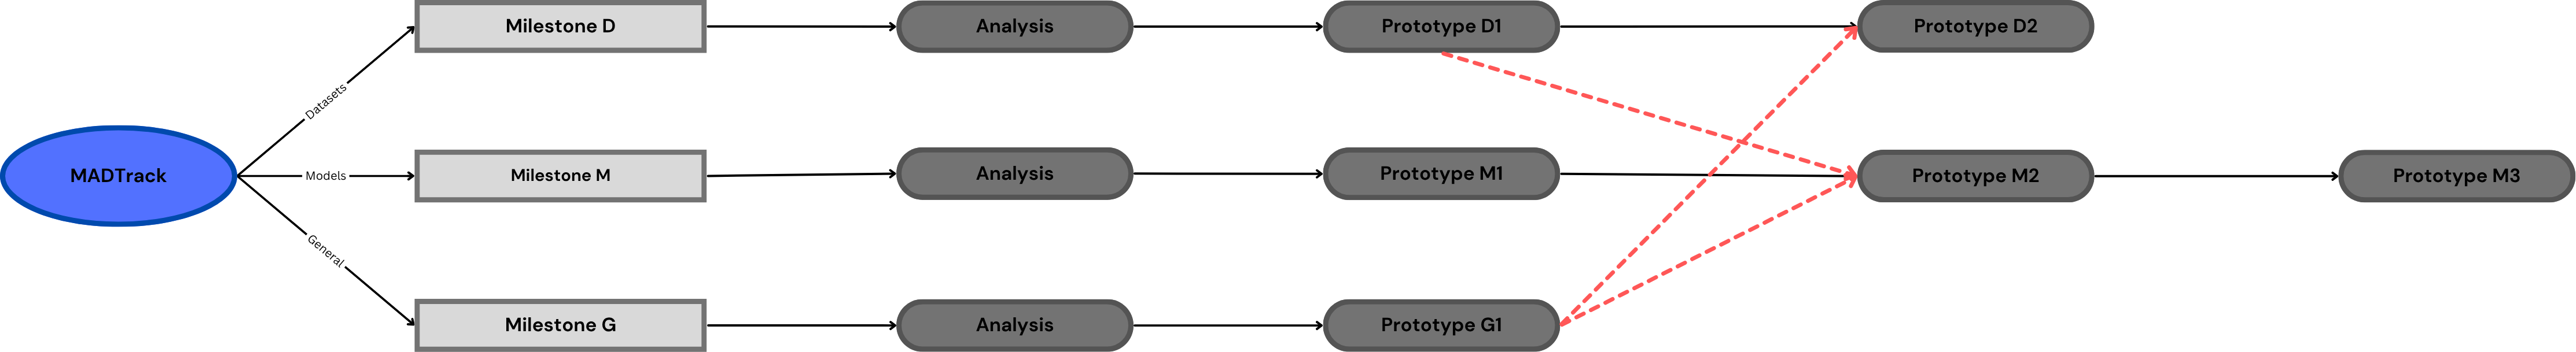
\includegraphics[width=\linewidth]{figs/MADTrack-roadmap.png}
    \caption{Iteration roadmap of the MADTrack project.}
    \label{fig:roadmap}
\end{sidewaysfigure}

\begin{sidewaysfigure}
    \centering
    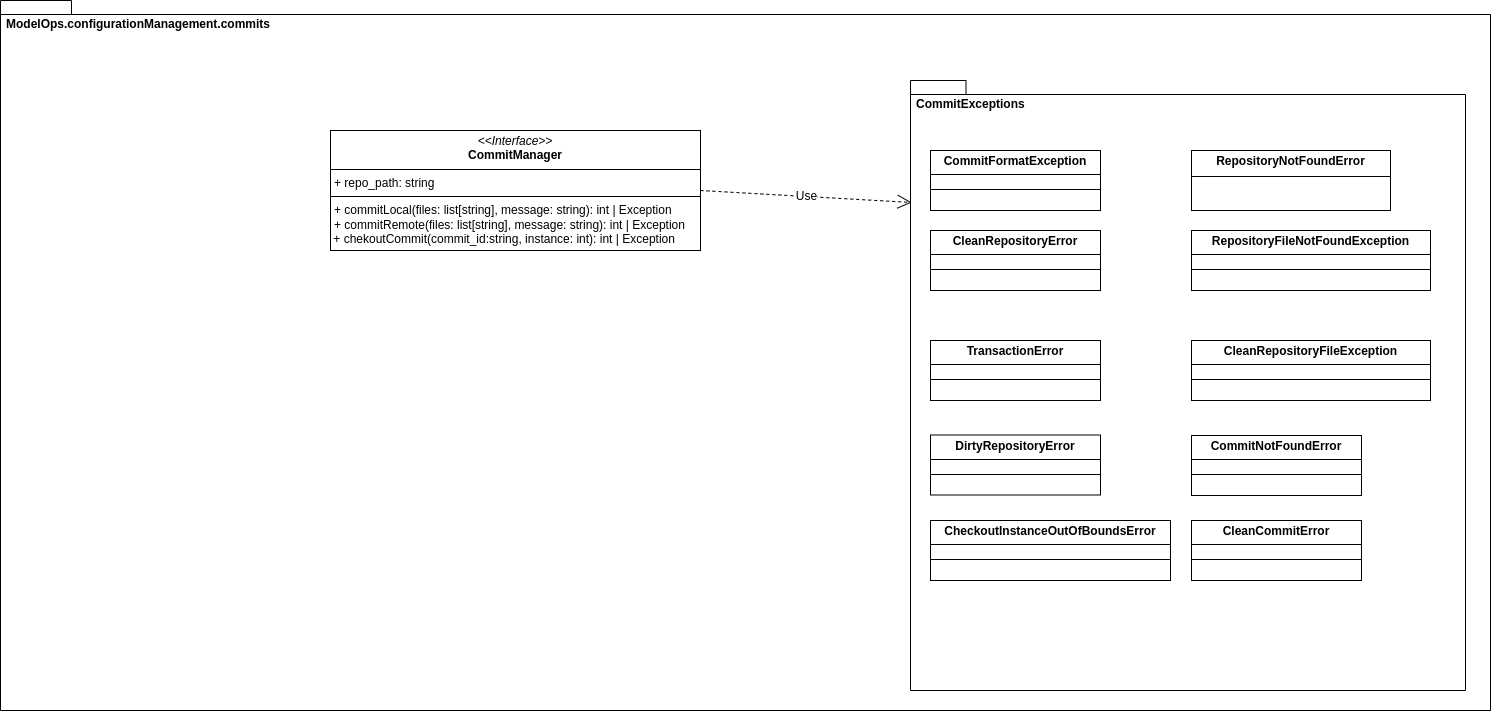
\includegraphics[width=\linewidth]{figs/G1-classDiagram.png}
    \caption{Class diagram for prototype \emph{G1}.}
    \label{fig:G1classDiagram}
\end{sidewaysfigure}
 % Apéndice A (opcionales)
\include{./Anexos/AnexoB} % Apéndice A (opcionales)
%--- (FIN DOCUMENTO)
\end{document}